\section{Hardware}

The hardware components of the system were selected for their cost and mobility. There are only two necessarily unique hardware components in the system, a Raspberry Pi 4 microcontroller and a Pi Cam, which are used a data collection node, capturing and processing video and then sending the road statistics away. Any retail laptop or computer is suitable for hosting the system's database and running the web-browser user interface.

\subsubsection{Node Hardware}

A computer suitable for performing the functionality required of a node has to be small, inexpensive, sufficiently powerful to run a computationally expensive algorithm, have networking capabilities and interface with a camera module. The Raspberry Pi 4 was selected for it meets all of these requirements and has the added benefits of a native operating system, support drivers for usb proprietary camera hardware and a large online community. It's ease of use due to these additional factors made the Pi an excellent choice for rapidly prototyping a computer vision system. 

The Pi Camera was the selected image capture hardware primarily for it's compatability with the Raspberry Pi environment but it is also inexpensive, can captures colour at a suitable resolution and frame rate. Figure \ref{fig:raspi_gear} shows the microcontroller with camera connected. Appendix \ref{appendices:hardware_specs} gives the full specifications of both of the Raspberry Pi 4 and Pi Cam.

\begin{figure}[H]
    \centering
    \centering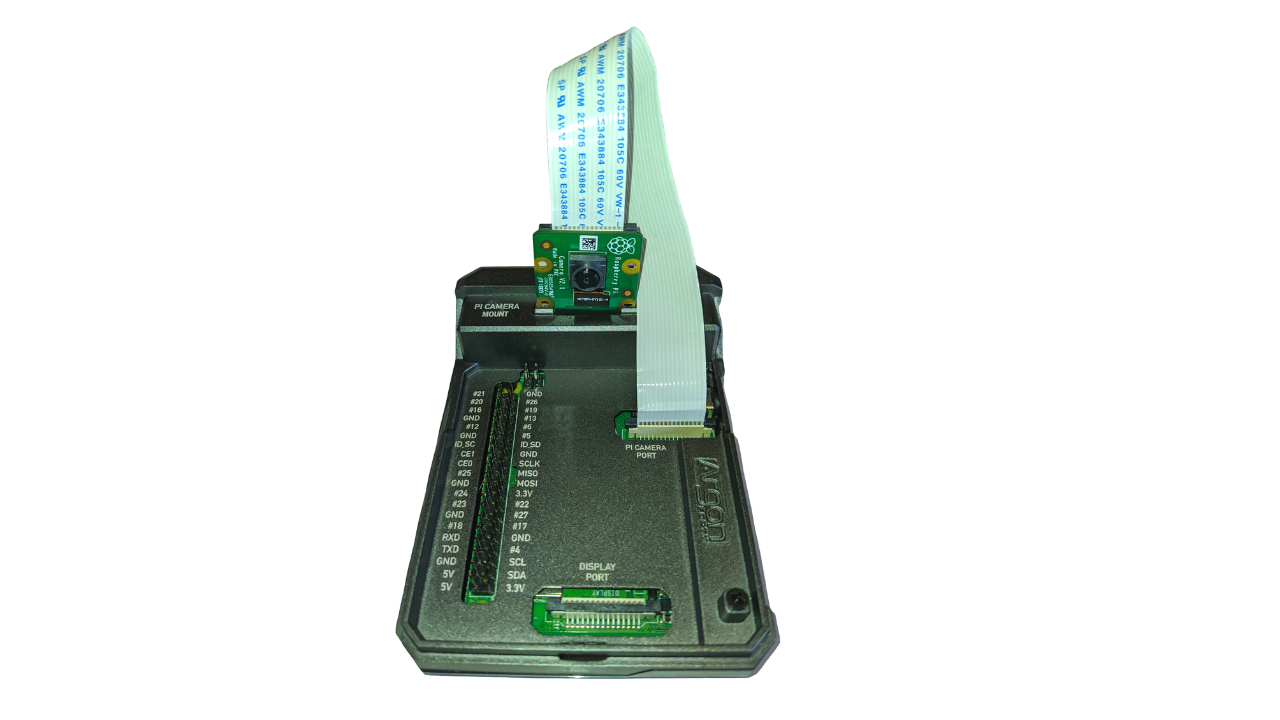
\includegraphics[width = 0.8\textwidth]{design/hardware/gear_improved}
    \caption{Raspberry Pi 4 and Pi Cam connected.}
    \label{fig:raspi_gear}
  \end{figure}
  